\section{Sphinx}\label{sec:sphinx}

Sphinx packets consist of a header and an encrypted payload. 
The header itself contains a \textit{cryptographic element $\alpha$} (e.g. $g^x$ or an elliptic curve point), \textit{encrypted routing information $\beta$}, and an \textit{integrity tag $\gamma$}, as illustrated in Figure \ref{fig:sphinx_structure}.

\begin{figure}[h]
    \centering
    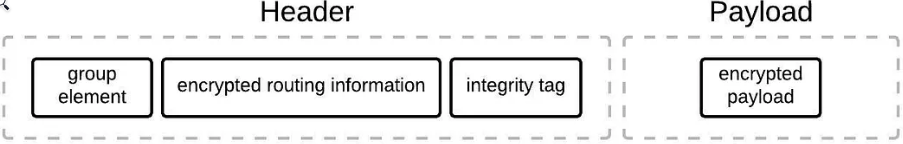
\includegraphics[width=0.9\linewidth]{Images/sphinx_structure.png}
    \caption{Structure of sphinx packet. \href{https://blog.nymtech.net/sphinx-tl-dr-the-data-packet-that-can-anonymize-bitcoin-and-the-internet-18d152c6e4dc}{[source]}}
    \label{fig:sphinx_structure}
\end{figure}

The \textit{encrypted routing information ($\beta$)} is constructed in layers, applied in reverse order along the path.
First, the final destination is encrypted, and an integrity tag ($\gamma_i$) is computed. 
The IP address of the last mixnode ($n_i$) is then prepended.
As shown by Figure \ref{fig:sphinx_header}, this process repeats iteratively: each new header is encrypted, an integrity tag ($\gamma_{i-1}$) is computed, and the IP address of the preceding mixnode ($n_{i-1}$) is prepended.
This layered encryption ensures that each mixnode can only decrypt its own layer, revealing the next forwarding address while preserving end-to-end confidentiality and protecting against tampering.

\begin{figure}[h]
    \centering
    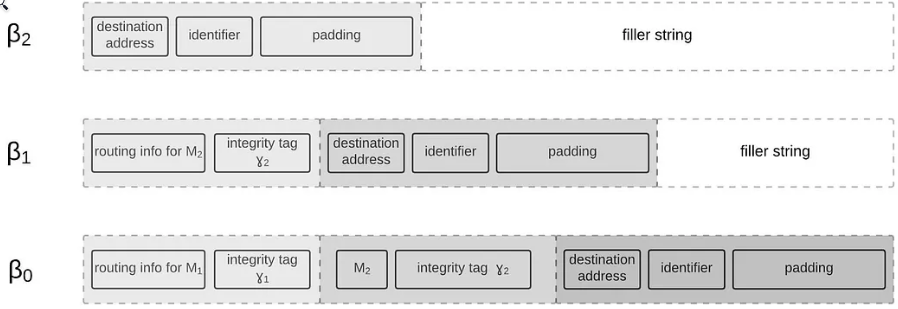
\includegraphics[width=\linewidth]{Images/sphinx_header.png}
    \caption{Sphinx encrypted routing information encapsulation. \href{https://blog.nymtech.net/sphinx-tl-dr-the-data-packet-that-can-anonymize-bitcoin-and-the-internet-18d152c6e4dc}{[source]}}
    \label{fig:sphinx_header}
\end{figure}

To encrypt the routing information, the Nym client\todo{previously "user" but JT prefers "Nym client"} first chooses a nonce $x$ and compute $\alpha = g^x$ as the \textit{cryptographic element} of the header.
Since each mixnode $i$ has a private key $x_i$ and a public key $y_i = g^{x_i}$, the user can create a shared secret $s_i$ with mixnode $i$ as followed: $s_i = y_i^x = (g^{x_i})^x$. 
Then the mixnode $i$ receiving the packet will get $\alpha$ allowing him to compute the shared secret as followed: $s_i = \alpha^{x_i} = (g^x)^{x_i}$.

Instead of sending a unique \textit{cryptographic element $\alpha$} at each node in the path, the sphinx format uses a single \textit{cryptographic element $\alpha$}, which is progressively modified at each node. 
Each mixnode updates the cryptographic element using its shared secret as follows:  
$$\alpha_{i+1} = \alpha_i^{\text{hash}(\alpha_i, s_i)}$$
Thus, the user iteratively computes the shared secrets in the path's order as: 
$$
\begin{aligned}
    \alpha_0 &= g^{x}, & s_0 &= y_{n_0}^{x}, & b_0 &= \text{hash}(\alpha_0, s_0) \\
    \alpha_1 &= g^{x b_0}, & s_1 &= y_{n_1}^{x b_0}, & b_1 &= \text{hash}(\alpha_1, s_1) \\
    &\vdots & &\vdots & &\vdots \\
    \alpha_i &= g^{x b_0 \cdots b_{i-1}}, & s_i &= y_{n_i}^{x b_0 \cdots b_{i-1}}, & b_i &= \text{hash}(\alpha_i, s_i)
\end{aligned}
$$
This formulation ensures that each mixnode can independently derive the necessary cryptographic elements without requiring the full path’s information, preserving privacy and unlinkability.  
\newline

The \textit{encrypted routing information ($\beta$)} is computed, as illustrated in Figure\todo{$\sim$\textbackslash ref\{\}} \ref{fig:sphinx_header}, by processing the path in reverse order. 
This involves XORing the routing information ($\beta_{i-1}$) from the previous layer (with the node's address and integrity tag) with a value derived from the shared secret $s_i$. 
Then prepending this new encrypted routing information ($\beta_i$) with an integrity tag ($\gamma_i$) and the previous mixnode address (remember we build it in reverse order).
We repeat the same process for each layer (i.e. each mixnode in the path).

\begin{figure}[H]
    \centering
    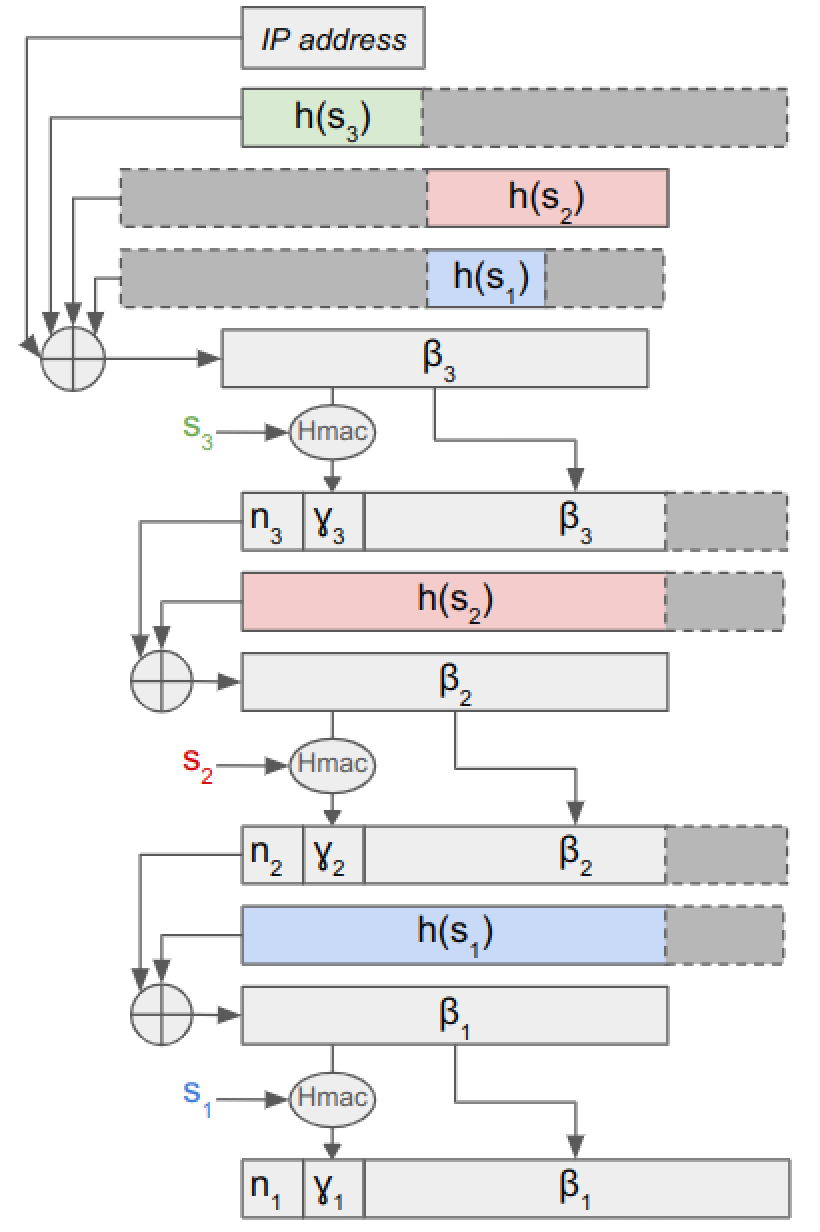
\includegraphics[width=0.5\linewidth]{Images/header_cipher.png}
    \caption{Construction of the Sphinx header (modified from \cite{sphinx}) [TO FIX: $h(s_1)$ at first XOR]}
    \label{fig:header_cipher}
\end{figure}
\todo[inline]{JT: Explain what the modifications are}
\todo[inline]{JT: Might help to put some (1) (2) (3) labels into the figure and refer to these labels in the text.}

% first round
The first round of XOR operations differs from the others because it requires combining parts of all shared secrets. 
Specifically, the destination address is XORed with the last node’s shared secret, truncated to match the address size.
Next, the result is concatenated with the XORed values of the ending parts of the shared secrets from the other nodes in the path. 
This ensures that when the entire header is XORed with the full shared secret, these appended values cancel out, allowing the header to be processed in reverse order by the mixnodes.
This design choice guarantees fixed-size headers, enabling fixed-size packets which is a crucial property in mixnets for maintaining unlinkability.

\todo[inline]{JT: Now maybe follow up with an example of the attack from the introduction?
We should also compare computational overheads from attack vs. the new protocol design.}
